
\section{Boyle's Law}

Name \rule{2.0in}{0.1pt}\hfill{}Section \rule{1.0in}{0.1pt}\hfill{}Date
\rule{1.0in}{0.1pt}

\textbf{Objective}

To investigate the relationship between the pressure and volume of
a gas.

\textbf{Apparatus}

\begin{itemize}
\item Boyle's law apparatus
\item Barometer
\end{itemize}
\vspace{0.3cm}
{\centering 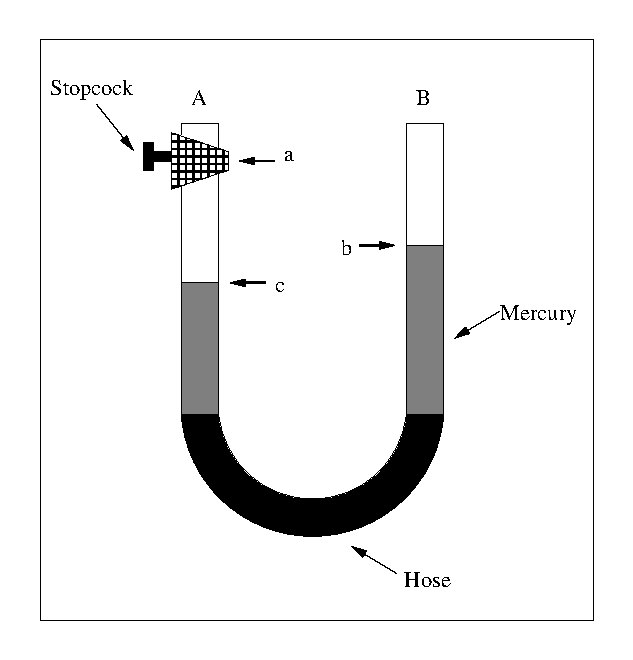
\includegraphics{boyles_law_fig_1.eps} \par}
\vspace{0.3cm}

\textbf{Introduction}

The behavior of a gas can be described in terms of the macroscopic
quantities: temperature (T), pressure (P), and volume (V). The relationship
between these quantities is given by the equation of state of the
gas. A real gas behaves approximately as an ideal gas if it is far
from liquefaction. In that case, the equation of state of an ideal
gas can be used to describe a real gas. For a given mass of a gas,
if one of the quantities P, T, or V is changed, a change in the other
two quantities probably will result. However, if one of the quantities
is kept constant, the relationship between the other two can be studied.
The relationship between pressure and volume of an ideal gas is called
Boyle's law.

The experimental apparatus is shown in the figure above. The gas is
air contained in tube A between points a and c. The temperature of
the gas will be that of the room and essentially constant. Between
points c and b the tube contains mercury. The pressure of the gas
is varied by raising or lowering the open tube B. The pressure is
numerically equal to atmospheric pressure, in cm Hg, plus the difference
in heights between points b and c (b - c). The volume of the enclosed
gas is the product of the cross-sectional area of tube A and the distance
between points a and c (a - c). Since the area is constant, the volume
is proportional to the length (a - c) = L.

\textbf{Note:} Do not tamper with the stopcock during the experiment
and make all readings before doing the calculations.

\textbf{Activity 1: Relationship Between P and V of a Gas}

(a) Determine and record in the space below the atmospheric pressure,
P\( _{atm} \), in cm Hg and the position of point a in cm.
\vspace{20mm}

(b) Construct a data table in the space below with the column headings:
b (cm), c (cm), b - c (cm), L = a - c (cm), 1/L (cm\( ^{-1} \)),
P (cm Hg), and PL (cm\( ^{2} \) Hg).
\vspace{120mm}

(c) Adjust the tube B so that b = c. Wait a few seconds for the gas
to come to thermal equilibrium with the surroundings, and then record
b and c in the data table.

(d) Lower tube B about 3 cm. Again wait for thermal equilibrium, and
then record points b and c in the table.

(e) Repeat step (d) until B is at the lowest position at which the
reading of points b and c can be obtained. Be careful that the hose
is not pinched in these lower positions.

(f) Now reverse the process. Raise B about 3 cm, wait for thermal
equilibrium, and record points b and c in the table.

(g) Repeat step (f) until b = c. If the final and initial positions
at which b = c do not coincide, consult your instructor.

(h) Calculate the total pressure P and the length of the gas column
L (which is proportional to the volume of the gas in tube A) for each
set of readings and enter these values in the table. Does inspection
indicate how they are related? Explain.
\vspace{20mm}

(i) Calculate and record the product PL for each set of readings.
Also, determine the mean value and the standard deviation \( \sigma  \)
for PL. Report the results below in the form PL = Mean \( \pm \sigma  \).
What does this result tell you about the product PL? What does it
tell you about the relationship between P and V? Explain.
\vspace{20mm}

(j) Create a graph of P (y axis) versus 1/L and fit the data to find
the mathematical relationship. Attach a copy of the graph to the unit.
What does this tell you about the relationship between P and V? Explain.
